% 20200713
\documentclass[../thesis.tex]{subfiles} %% use packages & commands as this main file
\begin{document}
\section{Result}
Among the four settings, phytoplankton-bacteria coexisting systems with harvest (PBH), the former without harvest (PBN), phytoplankton-only culture with harvest (PoH) and the former without harvest (PoN), top 10\% high yield scenarios showed PBH system yielded significantly more than others with 95\% confidence under a standardised temperature range of \temp\ (Fig.\ref{f:ydByPara}).  Pairwise Wilcox test showed that all four settings have significant pairwise yield flux distribution from one another (p $<$ 0.01).  All groups only reached its maximum yield flux at minimal phytoplankton intraspecific interference rate.

PBH systems had limited parameter ranges on five of the parameters (i.e. x, ePR, gP, aP and eBR) along the parameter range defined in this study.  With a median of 120.61 \dxdt) and an interquartile range (IQR) of [91.44-160.93] \dxdt, the group was the third in maximum yield flux (284.62 \dxdt) with the smallest sample size (n=326).  High harvest rate, high phytoplankton respiration fractions, low phytoplankton growth rate, non-minimal phytoplankton intraspecific interference and high bacterial non-respired carbon fraction made the system unfeasible.  Yield maximised at low harvest rate, high growth in phytoplankton biomass, density-insensitive phytoplankton death rate, mid-level carbon to biomass efficiency in bacteria, high bacterial growth rate and low bacterial death rate.

PBN systems had no parameter limitations across all parameter ranges.  Yet they yielded the worst in all scenarios.  With a median of 0.08 \dxdt and an IQR of [0.03-0.25] \dxdt, the group was also the last in maximum yield flux (246.28 \dxdt) with a moderate sample size (n=86538).  It had its maximum yield flux at very low harvest rate, moderately high phytoplankton non-respired carbon fraction, maximum phytoplankton biomass growth under high phytoplankton growth rate, moderately-high bacterial resource to biomass conversion efficiencies, high bacterial growth rate and moderate bacterial death rate.  

PoH systems had a median of 17.09 \dxdt and an IQR of [9.49-41.14] \dxdt.  The group had the highest maximum yield flux (345.75 \dxdt) with the largest sample size (n=110002).  Unfeasible scenarios occurred when phytoplankton had very low fractions of non-respired carbon, low growth rates and high intraspecific interference.  Fluctuations in yield on bacterial parameters were due to LHS sampling and extraction of top 10\% yield samples.  Yield maximised at very high harvest rate and high carbon to biomass fraction in high growth rate phytoplankton.

PoN and PoH systems behaved similarly in all parameter ranges although they were statistically different.  It had the same sample size with PoH (n=110002) and was the second-highest maximum yield flux (345.70 \dxdt).  Its median was 16.94 \dxdt\ and IQR was [9.43-40.99] \dxdt.  PoN had its parameter limits and maximum yield same as PoH systems except for the harvest rate parameter.  PoN has a slightly lower maximum harvest rate than PoH although their distributions overlapped.

\begin{figure}
    \centering
    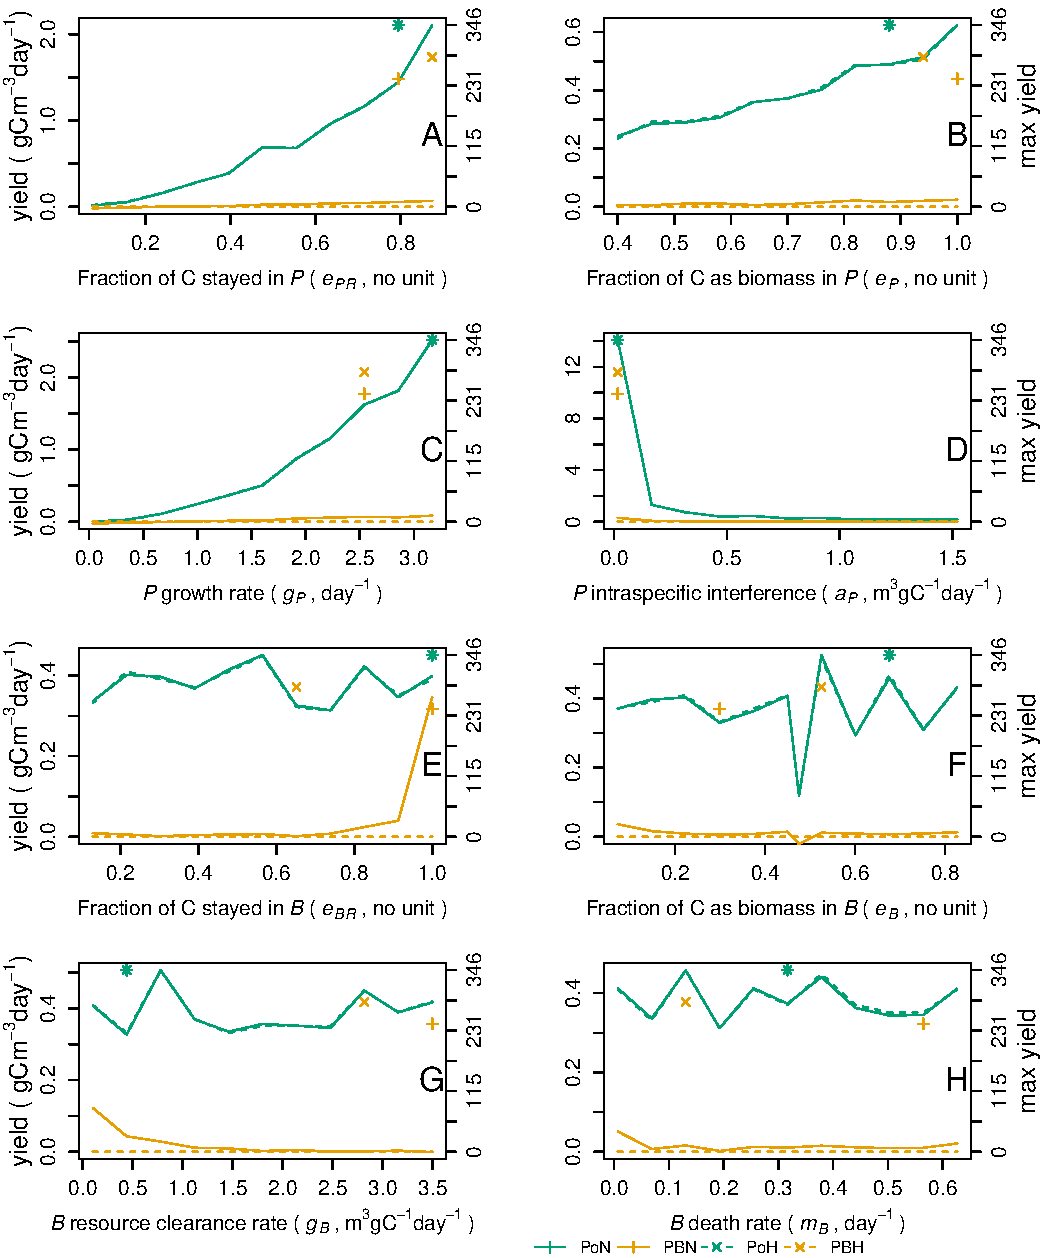
\includegraphics{result/yieldFlux.pdf}
    \caption{Yield flux distribution in parameter space.  Distribution of yield flux (\dxdt) with 95\% confidence interval was shown along respective parameter ranges under a standardised temperature range of \temp.  Top yield scenarios for each of the four settings (PBH, PoH, PBN, PoN) were plotted at its respective parameter values.  Orange solid lines/circles represented PBH systems (n=326) and its maximum scenario; orange dash lines/triangles represented PBN systems (n=86538); green solid lines/circles represented PoH (n=110002) systems; green dash lines/triangles represented PoN (n=110002) systems.  Shaded area around each line was the 95\% confidence interval for respective groups.  Pairwise Wilcox test showed that all four settings have significant pairwise yield flux distribution from one another (p $<$ 0.01).}
    \label{f:ydByPara}
\end{figure}

\end{document}